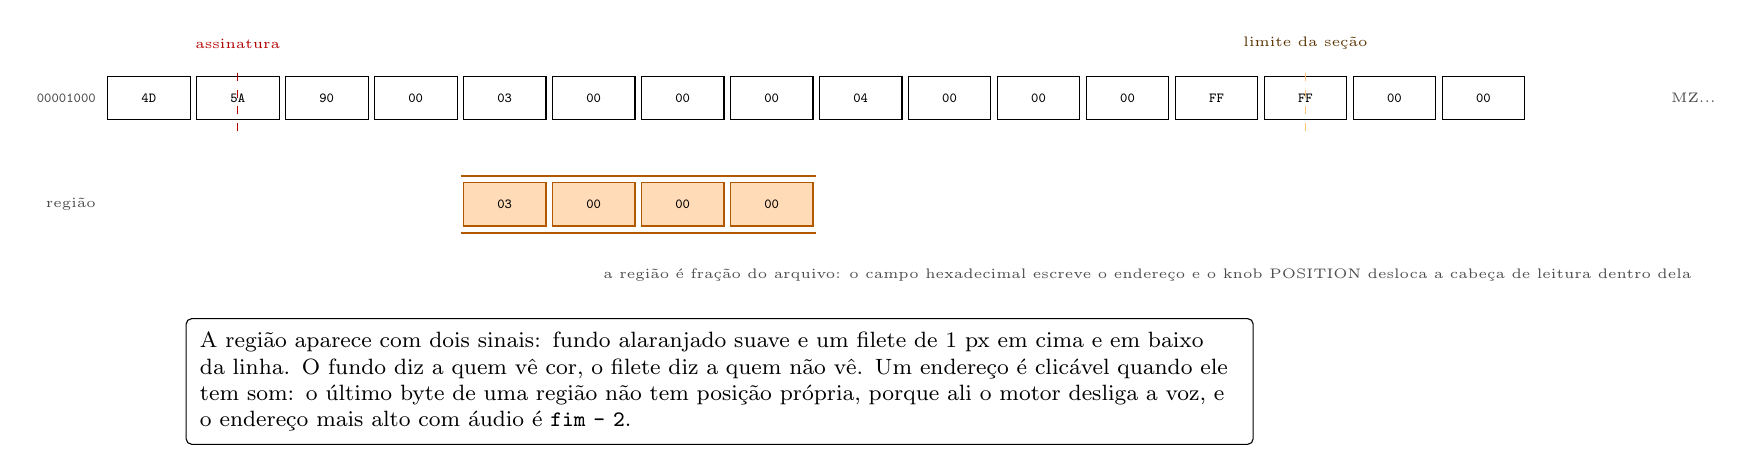
\begin{tikzpicture}
  \tikzstyle{cell}=[draw, minimum width=1.05cm, minimum height=0.55cm, font=\tiny\ttfamily, inner sep=1pt]
  \tikzstyle{lbl}=[font=\tiny, text=black!70]

  % linha de exemplo (endereco 0x1000)
  \node[lbl, anchor=east] at (0,0) {\texttt{00001000}};
  \foreach \i [count=\c from 0] in {4D,5A,90,00,03,00,00,00,04,00,00,00,FF,FF,00,00} {
    \node[cell] at ({0.55+\c*1.13},0) {\i};
  }
  \node[lbl, anchor=west] at ({0.55+17*1.13},0) {MZ...};

  % marcacao dos limites
  \draw[red!70!black, dashed] ({0.55+1*1.13},-0.42) -- ({0.55+1*1.13},0.42);
  \node[font=\tiny, text=red!70!black, anchor=south] at ({0.55+1*1.13},0.5) {assinatura};
  \draw[orange!85!yellow!55, dashed] ({0.55+13*1.13},-0.42) -- ({0.55+13*1.13},0.42);
  \node[font=\tiny, text=orange!85!yellow!35!black, anchor=south] at ({0.55+13*1.13},0.5) {limite da seção};

  % região destacada
  \node[cell, fill=orange!28, draw=orange!70!black] (r1) at ({0.55+4*1.13},-1.35) {03};
  \node[cell, fill=orange!28, draw=orange!70!black] (r2) at ({0.55+5*1.13},-1.35) {00};
  \node[cell, fill=orange!28, draw=orange!70!black] (r3) at ({0.55+6*1.13},-1.35) {00};
  \node[cell, fill=orange!28, draw=orange!70!black] (r4) at ({0.55+7*1.13},-1.35) {00};
  \draw[orange!70!black, thick] ({0.55+4*1.13-0.56},-1.35+0.36) -- ({0.55+7*1.13+0.56},-1.35+0.36);
  \draw[orange!70!black, thick] ({0.55+4*1.13-0.56},-1.35-0.36) -- ({0.55+7*1.13+0.56},-1.35-0.36);
  \node[lbl, anchor=east] at (0,-1.35) {região};

  % cabecas de leitura
  \node[lbl, anchor=west] at ({0.55+5*1.13},-2.25) {a região é fração do arquivo: o campo hexadecimal escreve o endereço e o knob POSITION desloca a cabeça de leitura dentro dela};

  % nota
  \node[draw, fill=white, rounded corners=2pt, align=left, font=\footnotesize, inner sep=5pt, text width=13.2cm] at (7.8,-3.6)
    {A região aparece com dois sinais: fundo alaranjado suave e um filete de 1 px em cima e em baixo da linha. O fundo diz a quem vê cor, o filete diz a quem não vê. Um endereço é clicável quando ele tem som: o último byte de uma região não tem posição própria, porque ali o motor desliga a voz, e o endereço mais alto com áudio é \texttt{fim - 2}.};
\end{tikzpicture}
